\documentclass[border=2pt]{standalone}
\usepackage[dvipsnames,svgnames,x11names]{xcolor}
\usepackage{tikz}
\usepackage{pgfplots}
\pgfplotsset{compat=1.18}
\usetikzlibrary{calc,arrows.meta,positioning,intersections,fit,shapes.geometric}
\usepgfplotslibrary{fillbetween}

\begin{document}
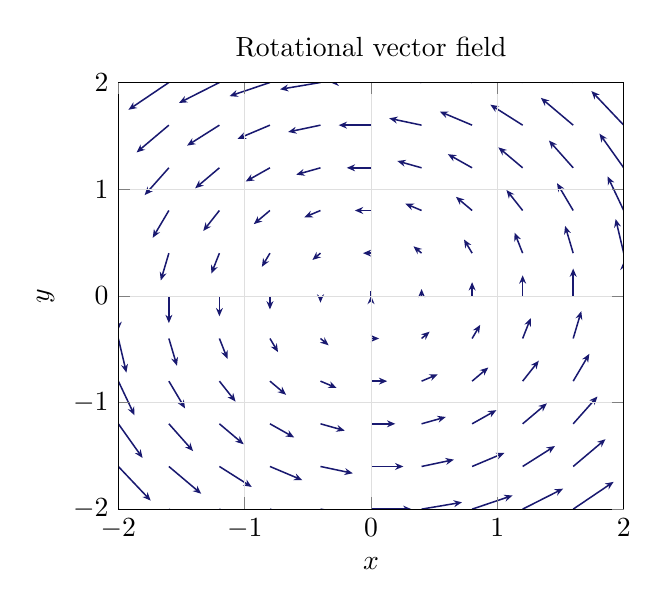
\begin{tikzpicture}
\begin{axis}[
  width=8cm,
  height=7cm,
  grid=major,
  grid style={gray!25,line width=0.2pt},
  title={Rotational vector field},
  title style={align=left},
  view={0}{90},
  3d box=complete,
  xlabel={$x$},
  xmin=-2,
  xmax=2,
  ylabel={$y$},
  ymin=-2,
  ymax=2,
  zmin=-0.1,
  zmax=0.1,
  legend style={draw=none,fill=none,cells={anchor=west}},
]
\addplot3+ [MidnightBlue,line width=0.55pt,mark=none,quiver={u={-y},v={x},w={0},scale arrows=0.16},-{Stealth[length=3pt,width=2.5pt]},domain=-2:2,y domain=-2:2,samples=11] {0};
\end{axis}
\end{tikzpicture}
\end{document}
